%%%%%%%%%%%%%%%%%%%%%%%%%%%%%%%%%%%%%%%%%%%%%%%%%%%%%%%%%%%
% EPFL report package, main thesis file
% Goal: provide formatting for theses and project reports
% Author: Yann Gabbud <yann.gabbud@epfl.ch>
%%%%%%%%%%%%%%%%%%%%%%%%%%%%%%%%%%%%%%%%%%%%%%%%%%%%%%%%%%%

\documentclass[a4paper,11pt,oneside]{report}
% Options: MScThesis, BScThesis, MScProject, BScProject
\usepackage[MScThesis,lablogo]{EPFLreport}
\usepackage{xspace}

\title{Secure, regulated and decentralized marketplace for the ticketing industry}
\author{Yann Gabbud}
\authorAddress{yann.gabbud@epfl.ch}
\affiliation{Distributed Computing Laboratory \\
and \\
Secutix SA, an ELCA company \\}
\supervisor{Mr. Denis Komarov}
\adviser{Prof. Rachid Guerraoui}
% \coadviser{Second Adviser}
% \expert{The External Reviewer}

\newcommand{\sysname}{FooSystem\xspace}

\begin{document}
\maketitle
% \makededication
\makeacks

\begin{abstract}
Players in the ticketing industry are constantly fighting against the black market and fraud to ensure that none of their customers are harmed by malicious people. In recent years, digital tickets based on blockchains have started to become more popular. The idea is to store tickets on the blockchain to guarantee their origin and integrity. Secutix has some experience in this area through their TIXnGO product. Two questions now arises. How to ensure that ticket resales are secure and regulated and how to build a decentralized ticket marketplace. \\

This thesis seeks to show that it is possible to build the foundations of a fully decentralized and regulated user management system, ticketing system and marketplace based on smart contracts, oracles and indexers. \\

We believe that our contribution is necessary because current solutions are mostly not decentralized or do not take full advantage of blockchain technologies. Moreover, having a regulated market is necessary and will certainly become the norm in the coming years when governments begin to regulate blockchain technologies. \\
\end{abstract}

\maketoc

%%%%%%%%%%%%%%%%%%%%%%
\chapter{Introduction}
%%%%%%%%%%%%%%%%%%%%%%
The ticketing industry is a big market which is expected to reach a capitalization of around 60 billion by 2026. Every year, people all over the world buy tickets for football matches, concerts or festivals. Unfortunately, sometimes they pay too much for a ticket or they buy fake tickets sold by dishonest people.

A ticket is usually a simple PDF with a QR code and some information such as the start time of the event or the location of the event. This PDF is generally sent by email to a spectator \footnote{You can find more info about the ticketing terminology \hyperref[sec:ticketing_terminology]{here}.} who prints it or keeps it on his phone. Once at the event, the spectator shows his ticket which is scanned by the staff. If the ticket is valid the spectator can enter.

This approach is very simple and practical to use for both the spectator and the organizer of the event. However, it is also very insecure. Indeed nothing prevents someone from buying a ticket and then reselling it to several different people. People who purchase the ticket have no way of knowing that there are multiple instances of the same ticket in circulation. Therefore, although the ticket is valid, only the first person who scans this ticket will be able to enter the event. Others will be refused entry because the ticket has already been scanned. Note, that it is even possible for a dishonest person to simply forge fake tickets that look deceptively like an original without buying one first.

One solution that event organizers use is to issue name tickets. As the ticket is nominative, it is impossible to forge a fake one. In addition, no one will want to buy a named ticket that is not in their name because they will be denied entry. While this mitigation works, it complicates a lot ticket reselling in secondary markets because each time someone wants to resell a ticket, the organizer must delete the old ticket and issue a new one which is really inconvenient.

Secutix SA, a famous player in the ticketing industry, started to develop in 2016 a new product called TIXnGO which aims to prevent fraud. The goal of TIXnGO is to replace traditional paper tickets with digital tickets recorded on a blockchain in a smart contract. Here is an overview of how it works. A user buys a ticket from an organizer. The user is invited to download the TIXnGO mobile application and to register by giving and verifying his email address. Once the user is registered, the digital ticket is created and injected into the smart contract. The smart contract saves the ticket and its owner. Finally, the user is notified that his ticket is available on the TIXnGO application. Once the day of the event has arrived, the user presents his smartphone to the access control which lets him enter.

This approach works very well to fight against fraud because only an organizer registered on TIXnGO can inject tickets on the blockchain. It is impossible for a malicious user to forge fake tickets and put them into circulation because the only way for him to do so is to register on TIXnGO and thus reveal his identity.

However, their approach is not sufficient because it is only partially decentralized and does not take full advantage of blockchain technology. Indeed, the blockchain is only used to store tickets. This certainly brings security and transparency, but a blockchain can be much more than a simple secure database. Moreover, their approach is custodial which means that users do not actually own their tickets and cannot use their own crypto wallet to store their tickets. Finally, this approach only partially addresses the problem of the black market. Indeed, nothing prevents a dishonest user from amassing numerous tickets and reselling them at high prices. To fight the black market, TIXnGO monitors all ticket movements to detect suspicious behavior. This is easy to do because all operations carried out on the blockchain are logged. Therefore, it is possible to know who is the original purchaser of a ticket, who is the current owner of a ticket and who were the previous owners of a ticket. TIXnGO analyzes this data and triggers alerts when illegal behaviors are detected. If necessary, measures are taken.

Ideally, the ticketing industry needs a user management system, a ticket management system and a marketplace that are fully decentralized, transparent, secure, and GDPR compliant. In addition, the marketplace must make it possible to easily resell tickets while allowing market regulation through transfer and resale rules \footnote{A resale rule is for example the resale price of a ticket cannot exceed more than 20\% of the initial price.} in order to fight the black market.

However, building such a system is not easy. The first challenge comes from the immutability of the logic of smart contracts. Once a smart contract has been deployed on the blockchain, it is no longer possible to modify it. This is a huge constraint because it means that all the logic, including the transfer and resale rules, must be planned in advance and cannot be changed later on. To change the logic, you must deploy a new smart contract with the new logic. You should know that deploying a smart contract can be very expensive. On the Ethereum blockchain, the cost of deploying a smart contract can go up to several thousand CHF in the event of heavy network congestion. Unfortunately, it is not possible to plan everything in advance because the logic and rules which were relevant in the past, will not necessarily be so in the future. Here is an example. In 2021 the English government imposed on event organizers to restrict the transfer and resale of tickets to only English citizens in order to limit the number of foreigners entering the country and therefore to fight against the spread of Covid19. This kind of event is typically impossible to anticipate. Therefore, to manage this new scenario it is necessary to deploy a new smart contract that supports the new constraints and so to pay again. It's really not practical in a real situation. We therefore need a system that is easily scalable.

The second challenge is the size of a smart contract. A smart contract cannot exceed a certain size limit. If this size is exceeded, it is not possible to deploy it. This therefore limits the complexity of the logic that a smart contract can have. The problem is that organizers have a lot of different logic and rules depending on the type of event or the location of the event. In addition, these rules may vary from one organizer to another. For instance, the organizers of the Wimbledon championships have defined more than a hundred different transfer and resale rules. It is clearly not possible to implement all of them in a smart contract. Note however that it is possible to cheat a bit by having a main smart contract calling secondary smart contract methods. However, although this trick allows for more richness in logic, it does not allow for arbitrary high complexity and the operating cost of such an approach is very high.

The third challenge comes from the fact that the blockchain, and therefore the smart contracts, do not have access to external data. Unfortunately, it is not possible to call a database from a smart contract. One solution would be to store all data directly on the blockchain. However, it would be extremely expensive. Moreover, according to the GDPR law, it is forbidden to store data concerning a user on the blockchain and the organizers themselves do not want some of their data to be public. Therefore, much of the logic simply cannot be implemented on a smart contract due to the lack of available data.

Finally, there are three other challenges that should also be mentioned. First, the system must be able to support a very large number of simultaneous operations. In one year, the system can manage up to several million tickets. This represents several thousand operations per day to be processed. Second, operation confirmation time must be relatively short. For example, when a ticket is scanned, the system must take it into account immediately so that it is not possible to enter the event twice with the same ticket. Finally, it must be possible to make complex and heavy queries about the state of the system. For example get all scanned tickets and sort them. Current blockchains are known not to be very good at these exercises at the moment. However, great progress has been made, in particular thanks to layer 2 such as zk rollups, which bring scalability without compromising security.

As it is not possible to implement and by extension to execute arbitrary complex logic on the blockchain, we suggest executing the logic outside the blockchain and verifying the result of the execution on the blockchain. To do this, we propose the following approach. The data necessary for the execution of the logic are stored on a database. The transfer and resale rules are also stored on a database. For each transaction, an oracle checks that the rules are respected. If this is the case, the oracle issues a proof that the transaction is authorized and therefore can be executed on the blockchain. When the user creates the transaction, he attaches the proof issued by the oracle. This proof is verified during the execution of the transaction. If the proof is not valid or has not been issued by the oracle, the transaction is refused. Otherwise, the transaction is executed.

With this approach, we can have smart contracts much simpler, supporting any rules of transfer or resale and less greedy in term of gas. Indeed, the smart contract only verifies that the proof is correct and does not need to execute a complex logic in order to approve or refuse the transaction.

Here is an example illustrating how our approach works. Suppose a spectator wants to resell a ticket. He bought it for 100 CHF and wants to resell it for 115 CHF. Suppose also, that the organizer of the event imposes that the resale price is not higher than 20\% of the initial price. As the resale price is less than 120 CHF, the resale is authorized. Here is the procedure. First, the spectator sends his request to the oracle which checks that the rules are respected. The request contains all the information that will be used to create the resale transaction on the blockchain, such as the identity of the buyer and the resale price. The Oracle uses the information contained in the request to create a transaction approval message, signs it and returns it to the user. The user creates the transaction with the information he has previously provided to the oracle and the approval message signed by the oracle. It sends the transaction to the blockchain which verifies it. The verification is ensured by a smart contract which knows the public key of the oracle. Finally, the transaction is executed.

Implementation and testing show that it is possible to build such a system and that it could be deployed in production. First, this approach is scalable. Indeed, an oracle running on a simple laptop easily supports 1,500 requests per second. The main bottleneck is still the blockchain. Second, verification on the blockchain of the oracle's message leads to a relatively small increase in transaction costs, on the order of 10\%. Note that if we were to run all the logic on the blockchain, the cost increase would be much higher. A simulation of the system on Polygon shows that the cost of performing a resale transaction is less than 1 cent, which is perfectly bearable for the ticketing industry or the users.

Therefore, this approach makes it possible to build a regulated market place that supports any regulation rules. In addition, as the execution is carried out or verified on the blockchain, we ensure a very high level of security and decentralization. The only downside comes from the oracle which is unfortunately not decentralized. However, decentralized oracles, such as Chainlink, exist and can be used to achieve a fully decentralized system.

In summary, our main contribution is to lay the foundations for building a secure, regulated and decentralized user management system, ticket management system and marketplace. We also offer other mechanisms that can be interesting for the ticketing industry such as time-based blockchain logic like automatically close an event once it is over or prevent ticket resale once an event has started. Finally, we want to clarify that although this approach uses the ticketing industry as a scenario, it can be perfectly applied to other sectors with similar needs.

%%%%%%%%%%%%%%%%%%%%
\chapter{Background}
%%%%%%%%%%%%%%%%%%%%
In this section, we introduce the background needed to understand this thesis. We first present the ticketing industry and the vocabulary it uses. Then we introduce the technologies and dependencies you need to know to understand the design and implementation.

\section{Ticketing terminology}
\label{sec:ticketing_terminology}

\begin{description} 
    \item \textbf{Digital Ticket}: A digital ticket is nothing more than a digital representation of a paper ticket. However, it has many advantages. First, it is more transportable and above all much more easily transferable or resalable than its paper counterpart. It is also more difficult to create fake digital tickets because they are generally cryptographically signed and governed by a system with an access control preventing anyone from putting them into circulation without first being approved. In our case, we use the ERC721 standard to represent digital tickets. This standard works well for digital tickets because it allows us to create unique transferable assets and keep track of who owns them.
    \item \textbf{Ticket wallet}: A ticket wallet is an application that stores digital tickets and displays them when requested by the user. In general, a wallet is a mobile application like the Apple wallet or a wallet dedicated to tickets like the TIXnGO wallet.
    \item \textbf{Event}: An event is a generic term that encompasses sporting events, festivals, concerts, or any other event that you need a ticket to attend.
    \item \textbf{Organizer}: An event organizer, or organizer for short, is a person or entity that creates, manages, and promotes events and sells tickets for them.
    \item \textbf{Spectator}: A spectator is someone who purchases tickets and attends events. A spectator may also transfer or resell tickets he has purchased from an organizer.
    \item \textbf{User}: Sometimes this term is used to encompasses both organizers and spectators who are registered in the system.
    \item \textbf{Ticket Transfer}: A spectator who owns a ticket can transfer it to someone else. This person becomes the new owner of the ticket. This change of ownership is called a ticket transfer.
    \item \textbf{Ticket Resale}: A spectator who owns a ticket can resell it to someone else. This is similar to a ticket transfer except that in addition to the ownership transfer there is also a money transfer. We say the current owner of the ticket is the seller and the person buying the ticket is the buyer. Therefore the seller transfers the ticket and the buyer transfers the money.
    \item \textbf{Transfer and resale rules}: Tickets are subject to transfer and resale rules defined by the organizer. These rules define a policy which mainly aims to fight against the black market and fraud. An example of a transfer rule might be that it is prohibited to transfer a ticket to a fan banned for hooliganism. An example of a resale rule might be that the resale price of a ticket cannot exceed more than 20\% of the original price.
    \item \textbf{Ticketing system}: A ticketing system, like Secutix, is a ticket management tool. An event organizer uses a ticketing system to create and manage events, to create, manage and sell tickets for an event, and to provide support and assistance to spectators who purchase tickets for its events.
    \item \textbf{Ticket Distribution System}: A ticket distribution system, such as TIXnGO, is a tool for managing the distribution of digital tickets. A ticket distribution system does not replace a ticketing system but is complementary. Often it also helps to fight against fraud and black market. In general, there are three main components. The first component is a management interface used by the organizer to distribute tickets purchased by spectators and to track who the current owners are. The second component is a ticket wallet which is used by the spectator to store, display, transfer and resell tickets. The third component is a backend which execute the requests of the organizers and the spectators. It is important to note that only a registered organizer can use the management interface. Therefore, only a genuine organizer can distribute tickets such that no fake tickets are in circulation.
    \item \textbf{Marketplace}: A marketplace is a platform that allows the secure sale of assets between parties that do not trust each other. In our case, the assets are tickets. The marketplace displays tickets that are on resale with their resale price. A seller can put a ticket up for resale and withdraw it later if they change their mind. A buyer can purchase a ticket on resale.
\end{description}

\section{Ethereum blockchain}
Ethereum is an open source blockchain \footnote{https://en.wikipedia.org/wiki/Blockchain} that runs smart contracts. It aims to be a global internet computer for building decentralized applications \footnote{https://en.wikipedia.org/wiki/Decentralized\_application}. It is currently the main blockchain used for DeFi \footnote{https://en.wikipedia.org/wiki/Decentralized\_finance}, NFTs and Dapps.

The system we design is based on the Ethereum blockchain. However, note that our implementation can be deployed on any EVM-compatible blockchain, such as Avalanche, Polygon or Binance smart chain. Note also that it is perfectly possible to implement the design so that the system can be deployed on blockchains that are not EVM-compatible but that support smart contracts such as Solana or Cardano.

\section{Ethereum wallet}
An Ethereum wallet is an application that let a user interact with the blockchain. With his wallet, the user can manage his account and assets. For instance he can get his ETH balance. He can make a transaction to transfer ETH to someone else. He can also connect and access to decentralized applications. A wallet stores a public and a private key. The public key is used to identify the account and by extension its owner. The private key is used to sign transactions and ensure that only the owner of the wallet can interact with his account. More information here \footnote{https://ethereum.org/en/wallets/}.

\section{Transaction}
A transaction is an operation initiated by an external account \footnote{https://ethereum.org/en/developers/docs/accounts/} that changes the state of the blockchain. An example of transaction is a transfer of ETH from one person to another. Since the transaction changes the state of the blockchain, the account that initiates the transaction must pay a transaction fee to the blockchain. In the example above, we see that the state of the blockchain is changed because the sender's account is decreased and the receiver's account is increased by the transferred amount. More information about transactions here \footnote{https://ethereum.org/en/developers/docs/transactions/}.

\section{Call}
A call is an operation on the blockchain that does not change the state of the blockchain. Both external and contract accounts can make calls. For example, one can make a call to get his ETH balance. Since a call is read-only, the call initiator does not have to pay any fees. More information about calls here \footnote{https://ethereum.stackexchange.com/a/770}

\section{Smart contract}
A smart contract, or contract for short, is a program that runs on the blockchain. As the blockchain is Turing complete, a smart contract can implement any arbitrary logic. However, there are two limitations to keep in mind. The first one is that a smart contract cannot call an external service and only has access to data that is stored on the blockchain or sent with a transaction. The second one is that a smart contract cannot implement arbitrary complex functions. Indeed if a function exceeds a certain complexity, the function will be reverted by the EVM \footnote{https://ethereum.org/en/developers/docs/evm/} because it exceeds the gas limit \footnote{https://ethereum.org/en/developers/docs/gas/#what-is-gas -limit }.

\section{ERC20}
ERC20 \footnote{https://ethereum.org/en/developers/docs/standards/tokens/erc-20/} is the Ethereum standard for creating fungible tokens. It defines a set of rules that must be implemented by any token wishing to be compatible with the standard. The main feature of such a token is fungibility. This means that the tokens are indistinguishable from each other. For example fiat currencies, such as CHF, EUR or USD. are fungible. Any CHF 100 note can be exchanged for another CHF 100 note. Stock auctions are also fungible. Thus, this standard aims to make it possible to represent any fungible asset on the Ethereum blockchain. 

\section{ERC721}
ERC721 \footnote{https://ethereum.org/en/developers/docs/standards/tokens/erc-721/} is a standard for non-fungible tokens. Like the ERC20 standard, ERC721 is a very popular standard. However, it has a different purpose. It aims to represent any non-fungible asset on the Ethereum blockchain. A non-fungible asset can be, for example, an event ticket. Indeed, each ticket has a unique identifier (UID) that distinguishes it from any other ticket for the same event. The Venus of Milo is another example of a non-fungible asset. There is only one Venus that was sculpted by Paros.

\section{Smart contract event}
An event is an information that can be emitted and logged by the blockchain when a transaction is mined. For example, when someone transfers ERC20 tokens, a \textit{Transfer} event is emitted. This event includes the following information: the sender's address, the receiver's address and the amount sent. Events emitted by a smart contract can be used to build indexes to perform complex data queries.

\section{Keccak256}
Keccack256 is one of the most widely used hash functions in the Ethereum ecosystem. This hash function is used in the EVM and in Ethash, the PoW algorithm of Ethereum. Note that this hash function is named keccak256 and not SHA3 \footnote{https://en.wikipedia.org/wiki/SHA-3} even though they are nearly identical. The reason is that keccak256 is an old version of SHA3. SHA3 was slightly modified in August 2015, right after the launch of Ethereum in July 2015. In our system, the oracles use keccak256 to calculate the approval message from user inputs.

\section{ECDSA}
ECDSA, Elliptic Curve Digital Signature Algorithm, is an algorithm used to digitally sign messages. This algorithm is very suitable for blockchains because, compared to its counterparts such as RSA, it uses shorter keys, it has faster signing and encryption operations and it offers the same level of security. Oracles use ECDSA to sign the messages they computed with keccak256.

\section{Blockchain oracle}
As mentioned earlier, smart contracts do not have access to data stored outside of the blockchain. Therefore, blockchain needs a way to bring data securely onto the chain. This is the role of an oracle. It guarantees the authenticity and integrity of this data so that the blockchain can access off-chain data securely without compromising its security.

\section{Graph protocol}
The Graph \footnote{https://thegraph.com/docs/en/about/introduction/} is a protocol used to index blockchain and smart contracts. It is very useful because it allows to build and maintain off-chain indexes tracking the state of the blockchain or smart contracts. Building an off-chain index is very useful because it simplifies access to information and reduces the complexity of smart contracts. There is no need to create and maintain complex data structures in the smart contract in order to be able to query arbitrary data, such as getting all balances of an ERC20 contract above a certain amount. It also allows to query data in bulk, which is not possible with a blockchain call due to the gas limit. Note that indexes are stored in a traditional database such as Postgres.

%%%%%%%%%%%%%%%%%%%%%%
\chapter{Related Work}
%%%%%%%%%%%%%%%%%%%%%%

\textit{The related work section covers closely related work. Here you can highlight
the related work, how it solved the problem, and why it solved a different
problem. Do not play down the importance of related work, all of these
systems have been published and evaluated! Say what is different and how
you overcome some of the weaknesses of related work by discussing the 
trade-offs. Stay positive!
This section is usually 3-5 pages.} \\

Many projects seek to create blockchain-based digital tickets and marketplace such as B.A.M, Blocktix. EventCHI, FanDragon, PassageX, TicketHash, TIXnGO or GET protocol. For most of them, it's not easy to find out how they work because they don't have documentation open to the public and the product description is aimed primarily at the marketing guys. What we can say is that they all offer a simple form of regulation such as limiting the maximum resale price in order to fight against the black market. They all have a custodial model, i.e. they handle tickets for users. They do not appear to be decentralized and primarily use blockchain as ticket storage.

We detail two systems similar to ours which seem to be the most promising and whose documentation is available: TIXnGO and GET Protocol. We begin by giving a description of these system. Then we explain what is different about our approach and how we overcome some of their weaknesses.

Let's start by explaining what these two systems do. They are both ticket distribution systems. TIXnGO is developed by Secutix SA and GET Protocol is developed by GUTS ticketing. Their approach is to use the blockchain to securely and transparently store tickets and their owners. Here's how it works. Take for example Fifa which organized the Arab Cup last year. First, Fifa sells tickets to spectators. Once the tickets are sold, it sends to the distribution system a list of tickets with their owner and the ticket details. The distribution system saves everything in a database and saves ticket ID and spectator ID pairs on the blockchain in a smart contract. Once done, it notifies spectators that their ticket is available on the mobile application. Once the tickets are in their possession, spectators can transfer their ticket to other registered spectators. When the day of the event is here, spectators scan their ticket at the entrance and enter the stadium.

Let's now take a closer look at TIXnGO. The approach fulfills its role well and the partners are very happy with the product. However, there are many things that we believe can be improved. The first point concerns the blockchain. TIXnGO uses its own private blockchain hosted on Amazon servers. Having a private blockchain is very convenient because there are no transaction fees to pay and it is possible to easily correct errors of manipulation as well as a bug in the code. However, a private blockchain doesn't make much sense because no one except TIXnGO has access to it. Organizers and spectators use the TIXnGO API but never communicate directly with the blockchain. Therefore most of the interesting properties of the blockchain such as transparency or direct management of assets by users are lost. To overcome this problem, our approach is based on a public blockchain.

The second point concerns business logic and general design. All the business logic of TIXnGO is managed off-chain by the backend, except the ownership of the ticket which is managed by the blockchain. This approach is very practical because it is much easier to have a business logic off-chain than on-chain. Indeed, there are many constraints such as smart contracts which cannot have an arbitrarily large complexity. In our opinion, it would be interesting to let the blockchain take care of the business logic because it would make it possible to really take advantage of the blockchain and not to use it simply as a database which is certainly very secure but which is also very expensive to operate. This would also make it possible to have a much more decentralized system and avoid a single point of failure. Our approach is to execute as much of the business logic as possible on-chain. The business logic that cannot be executed on-chain is executed off-chain and then checked on-chain. To do this we use oracles, smart contracts and indexers.

The third point concerns standards. TIXnGO uses homemade smart contracts that could be replaced by standards in order to avoid reinventing the wheel. There are several very useful standards, which have been extensively tested and are used by many projects. For example, it would be interesting to use the ERC721 standard to represent tickets and to keep track of their owner. The problem for TIXnGO is that it requires many system adjustments because at the moment it does not use Ethereum addresses as identifiers for users but database IDs. Our approach tends to use as much as possible the current standards in order to benefit from the work carried out by the blockchain community and to maximize the interoperability of our system with other projects.

Finally, although TIXnGO allows the resale of tickets, it does not have yet a marketplace. We propose to build such a fully decentralized marketplace allowing secure and regulated resales of tickets.

Now let's take a closer look at GET Protocol and compare it to TIXnGO. Note that as the systems are very similar, we will not go into detail so as not to repeat what has been said above. The first point to mention is that unlike TIXnGO, it is deployed on Polygon, a public blockchain. The second point to mention is that it makes somewhat better use of the blockchain. In addition to storing tickets on the blockchain, it stores events on the blockchain. This is very practical because it allows to effectively filter tickets by event. However, we feel that like TIXnGO, the system does not take full advantage of what the blockchain has to offer. The third point to mention is that it uses the ERC721 standard to represent tickets on the blockchain. Due to the popularity of this standard, this is a very good idea because it allows to have a system that can easily interoperate with other systems. Finally, like TIXnGO, it does not yet have a decentralized marketplace.

To conclude, we must briefly mention Taurus, a fast-growing Geneva startup. Taurus offers financial market infrastructure services and products such as a custody solution used by swiss bank. This solution allows banks to offer their customers the possibility of buying crypto assets. On top of that, they are building a regulated market, named TDX, to enable the trading and exchange of tokenized securities which is an essential and missing piece in the financial ecosystem and the first in the world as far as I know. The marketplace complies with Swiss securities law and Distributed Ledger Technology (DLT) law.

Although the business is different, it is interesting to see that another actor seeks to regulate decentralized assets as we seek to do. Unfortunately, there is no documentation and the API is not yet available. Therefore, it is difficult to understand how it works under the hood, except that it is custodial.

%%%%%%%%%%%%%%%%
\chapter{System overview}
%%%%%%%%%%%%%%%%

\textit{Introduce and discuss the design decisions that you made during this project.
Highlight why individual decisions are important and/or necessary. Discuss
how the design fits together.
This section is usually 5-10 pages.} \\

In this chapter, we first enumerate the goals that the system must achieved. Then, we describe the system and the design choices that were made. 

\section{System goals}

NFTiX offers the following benefits in terms of decentralization, scalability and security.

\begin{description}
  \item \textbf{Regulated Market}: NFTiX offers a mechanism to control the resale process so that the black market is limited.
  \item \textbf{Decentralization}: Expect oracles, there is no single point of failure in NFTiX such as a trusted third party.
  \item \textbf{High Throughput}: NFTiX supports thousands of daily operations (ticket issuance, transfer, resale, etc.)
  \item \textbf{Low Latency}: NFTiX offers low latency transaction confirmation.
  \item \textbf{Low Costs}: The operating cost of NFTiX is low for NFTiX developers, event organizers and spectators.
  \item \textbf{Ticket integrity, authenticity, tampering}: NFTiX ensures a high level of security so that the integrity, authenticity and unforgeability of tickets is guaranteed and no fraud is possible.
\end{description}

\section{Architecture overview}
This section aims to provide an overview of the main components and their interoperability. You can find more details about the components in the following sections.

\includegraphics[width=\textwidth]{architecture_overview.png}

\section{Oracles}
Oracles play a crucial role in the system. The Oracle Identifier and Approver allow us to execute business logic outside the blockchain and verify the result on the blockchain. The Price feed oracle is used to securely bring the price of TIX against USD and ETH on the blockchain.

It should be noted that the oracles all have a pair of private/public keys. These keys are used to sign transactions and messages.

We explained previously that a signed message was returned by an oracle if the operation is approved. We also call this signed message a proof because the oracle proves that it has done its due diligence. Now let's see how this message is created. Creation takes place in two phases. The first is to hash the arguments supplied by the user. To do this, the keccak256 hash function is used. Once the hash of the arguments has been calculated, the oracle creates the signature from the private key of the oracle and the hash thanks to ECDSA.

\subsection{Identifier}
The Identifier oracle makes it possible to verify the identity of organizers and spectators who wish to register, to store user information on the database and to issue identification proofs allowing users to register on the Identity contract.

At the moment, the oracle only verifies the Ethereum address that the user provides. To do this, the oracle sends a challenge that the user must sign and return to the oracle. The verification is successful if the Oracle manages to verify that the message has been signed by the private key corresponding to the address provided by the user. Note that, as the name suggests, the oracle should also verify the identity of the user. The verification mechanism is not implemented because outside the scope of the project. We therefore assume that the oracle performs an identity verification similar to that carried out during the onboarding of Coinbase, Binance or Swissborg, i.e. the user sends photos of his identity card and his face which are then verified thanks to machine learning.

Once the verification is successful, the oracle saves the information that the user has provided and issues a proof of identification built from the Ethereum address and the group to which the user belongs.

\subsection{Approver}
The Approver Oracle is responsible for verifying that all ticket transactions initiated by spectators comply with the rules imposed by the organizers and for issuing proofs of approval allowing spectators to carry out resale and swap transactions.

For a resale transaction, the proof is built from the address of the ticket owner, the token ID, the resale price and the address of the optional buyer. For a swap transaction, the proof is constructed from the address of the ticket owner, the token ID of the ticket offered, the event ID of the wanted ticket and the address of the optional buyer. Note that if the optional buyer is not specified, address zero is used to construct the proof.

The approbation procedure of a transaction works like this. First, the spectator sends a transaction approval request to the Approver oracle providing it with the data that will be used to construct the transaction. The oracle verifies that the transaction respects the rules and issues the proof of approval. The spectator constructs the transaction with the data that he transmitted to the oracle and with the proof that the oracle returned to him. Finally, it sends the transaction to the blockchain which will be processed by the Exchange smart contract.

\subsection{Price feed}
The price feed oracle regularly sends the price of TIX against USD and ETH to the TIX smart contract. As a reminder, smart contracts cannot communicate with the outside world and therefore the TIX smart contract has no way of knowing the price of the TIX if it is not transmitted to it.

This oracle works differently from the other two oracles. It communicates directly with the blockchain and therefore does not need to issue proofs. Indeed, as the transactions that the oracle sends are signed, the smart contract only needs to verify that the initiator of the transaction is the price feed oracle in order to ensure that the price update is legitimate. Note that the TIX smart contract stores the address of the oracle in order to verify that the transaction comes from it and not from a malicious user.

\section{Graph node}
The graph node execute the graph protocol. It allows us to make complex data requests that would be very difficult to do directly on the blockchain.

Let's start by understanding why it is difficult to do complex queries on the blockchain. There are two major limitations. The first is the gas limit. Indeed, like transactions, calls cannot have a complexity exceeding a certain limit. If the size of the returned data is too large, the call fails. However, this limitation is easily overcome if the data is simple. All you have to do is split a large query into several sub-queries. For example, if we want to obtain the balance of all the accounts of an ERC20 contract, we can query the first 100 balances in a first request, then the following 100 in a second request and so on. This requires two data structures on the smart contract, a list and a hashmap. The list stores users' balances and the hashmap maps a user's address to their balance's position in the list. This approach makes it possible to update a user's balance because the position of his balance is tracked by the hashmap and it is also possible to return all the balances by iterating over the list.

With this approach, it is also possible to easily create simple filters. Let's go back to the previous example and assume that the smart contract stores two additional hashmaps. The first hashmap tracks premium accounts and the second hashmap tracks VIP accounts. If we want to get the balance of all premium and VIP accounts, we can simply iterate over the list of accounts and return only the accounts tracked by one of the two hashmaps.

However, this approach is very limited because it is not possible to create queries as complex and rich as SQL would allow. There is not built-in primitive such as merge, join or filter to manipulate data. Therefore, if one wants to implement a complex query on a smart contract, he needs to implement by himself all these primitives. The code of the function would be very complicated to write and the request would fail as soon as the number of data becomes too large because the maximum gas limit would be reached.

The graph overcomes this limitation by creating an index outside the blockchain. The index is built through event emitted by transactions and can be queried through graphql \footnote{https://graphql.org/} queries.

Here is an overview of how the indexing works. Let's take for example an ERC20 contract storing the balance of users. When a user transfers tokens to another user, he first creates a transaction with the following fields: his address, the recipient's address and the amount he wants to transfer. The user sends the transaction to the blockchain which executes it. When the transaction is mined an event containing the three preceding fields is emitted and logged. The graph node listens to this event and updates its index by decrementing the sender's balance and incrementing the receiver's balance. You can find an overview in the figure \hyperref[fig:graph_node]{ \textit{Graph node}}.

\begin{figure}[h!] 
  \centering
  \includegraphics[scale=0.6]{graph_node.png}
  \caption{Graph node}
  \label{fig:graph_node}
\end{figure}

Now that we understand why it is difficult to make complex queries or obtain bulk data, let's look at its use in our system. The graph node maintains three indexes. The first stores all user information, i.e. address, group, balance in TIX, TIX allowance to Ticketing contract, TIX allowance to Exchange contract (only for the spectator). The second stores all event information, i.e. event ID, organizer, name, location, opening date and time, closing date and time, state, number of tickets. The third stores all ticket information, i.e. token ID, ticket ID, event ID, owner, state, status (on swap / on resale). To build and maintain these three indexes, the graph node listens to events sent by the four smart contracts. The list of events can be found in the \hyperref[sec:appendix_a]{Appendix A}.

\section{Database}
The database has three uses. It stores the data of the organizers and the spectators, i.e. the name, the first name, the address of residence, the email address and the Ethereum address. It stores the transfer and resale rules as well as the data necessary for their application. Finally, it stores the indexes created by the graph protocol.

TODO: graph node, marketplace, identifier, approver

\section{Ethereum blockchain}
The Ethereum blockchain is the cornerstone of the system. It is it who is responsible for operating the smart contacts that implement the business logic.

This component must be robust and battle tested to ensure that the execution environment is safe. We chose Ethereum because it is the most mature blockchain at the moment. It has been tested extensively. It hosts many projects. And it has a complete development and test environment.

However, it has a big disadvantage, the high cost of transaction fees induced by the congestion of its network. Unfortunately, it suffers from its popularity. However, many scalability solutions are under development and things should improve. In the meantime, it is possible to deploy the system on Polygon which is EMV-compatible and which offers a good level of security.

\section{Smart contracts}
This section describes the core of NFTiX which is responsible for applying the business logic. The core is made up of four interacting smart contracts, the Identity contract, the TIX contract, the Ticketing contract and the Exchange contract. We describe two versions: the initial version and the upgraded version. The initial version is the implementation of the initial design we made. The initial design contains a few mistakes that have not been detected during the design phase. The upgraded version fix these problems.

\subsection{Initial design}

\subsubsection{Identity smart contract}
The Identity contract allows organizers and spectators to register and unregister from the system. It allows NFTiX to revoke a organizer or a spectator who behaves inappropriately. It stores the addresses of registered organizers and spectators. It stores the Identifier oracle's public key so that it can verify the signature of approval messages issued by the oracle when an organizer or spectator registers. You can find the flow diagram of the user registration in the figure  \hyperref[fig:user_registration]{ \textit{User registration}}.

\begin{figure}[h!]
  \includegraphics[width=\textwidth]{user_registration.png}
  \caption{User registration}
  \label{fig:user_registration}
\end{figure}

This contract defines and applies the role-based access control policy. For now, the policy is very simple but it can be extended as needed. There are four roles: ORGANIZER, SPECTATOR, UNREGISTERED and REVOKED. An organizer who registers gets the ORGANIZER role and a spectator who registers gets the SPECTATOR role. When an organizer or spectator unregisters, their address is marked as UNREGISTERED. If NFTiX bans a user from the system for inappropriate behavior, the address is marked as REVOKED.

\subsubsection{TIX smart contract}
This contract manages the utility token of NFTiX, the TIX token. This contract is ERC20 compliant. The TIX is used to pay platform usage fees and to purchase resale tickets. Indeed, the platform generates revenue through the activity of its users. For example, when an organizer creates an event, he must pay a creation fee. Or, when a resale is made, a percentage of the resale is taken and shared between the event organizer and NFTiX.

The contract stores the price of TIX against dollars and ETH. These prices are regularly updated by the price feed oracle. The smart contract also stores the public key of this oracle so that only it can update the prices.

Users can request the current price of TIX against dollars or ETH. They can ask how many tokens an amount in dollars or ETH is worth. They can also buy TIX with ETH or sell TIX and receive ETH in return. When buying, TIX are minted and when selling, TIX are burned. Finally, the admin of NFTiX can request the ETH balance of the contract and remove or add ETH in the smart contract.

It is important to note that the token has no real use in itself because we could very well use ether instead. However, it does show to Secutix SA how a utility token can be integrated into the system and used by users. You will find more information on the potential use of the token in the future work section.

\subsubsection{Ticketing smart contract}
This contract manages events and tickets. As the tickets are represented by NFTs, the contract complies with the ERC721 standard.

Let's start by detailing the events. Events are represented by a data structure containing the following fields: an event ID, the address of the organizer, the name of the event, the place, the opening date and time, the closing date and time and finally the state of the event. 

Three of these fields serve useful purposes for business logic: the event ID, the opening date and time, and the state. The others could be stored off-chain to reduce gas consumption. The event ID is used to distinguish events from each other. This identifier is unique. The opening date and time corresponds to the opening of the doors of the event. This information is used to prevent transfers and resales of tickets after the opening of the event. This measure is necessary to prevent a malicious person from trying to resell a ticket that has already been scanned.

There are three possible states for an event. The first state is PENDING. This state means that the event has been created but that it is not yet open. Therefore, an organizer can create tickets for this event. However, it is impossible to transfer or resell them. The second state is OPEN. This state means that the event is activated. Therefore, spectators can transfer and resell their tickets. The last state is CANCELED. This state is obtained when an event is cancelled. Like the PENDING state, it allows transfers and resale to be frizzed. Although these two states have the same effects, it is useful to be able to distinguish them in order to filter events and tickets.

Now let's take a look at tickets. A ticket is made up of four fields: a token ID, an event ID, a ticket ID and a state. The token ID is the unique identifier that distinguishes NFTs from each other. The event ID is the event the ticket belongs to. The ticket ID is a unique identifier that allows the organizer to distinguish his tickets. Note that two organizers can share the same ticket ID. Therefore, to uniquely identify a ticket, you must either know its token ID or its ticket ID and its event ID. Finally, like an event, a ticket has a state. The first state is VALID. This means that the ticket can be transferred, resold or used to enter the event. The second state is INVALID. This means that the ticket has been invalidated by the organizer. There can be several reasons for this. It's a test ticket. Its bearer tried to defraud and its ticket was deleted. Or the ticket was canceled for another reason. The last state is SCANNED. This means that the ticket is valid and that the bearer has entered the event. This state is useful because sometimes it is necessary to scan a ticket again in the event, for example, to access the VIP area.

Let's now look at the interaction of organizers and spectators with the smart contract. First, it should be noted that some smart contract methods, such as event creation, can only be performed by an organizer. If a spectator attempts to execute one of these methods, the transaction will be reverted. To apply this restriction, the smart contract queries the Identity smart contract to find out if the initiator of the transaction is an organizer. Secondly, it should be noted that an organizer can perform an operation, for example minting a ticket, only if it is related to one of his events. If an organizer tries to interact with assets that they don't own, the transaction is reverted.

An organizer can interact with the contract to register an event. To do this, he must provide all the fields listed above and pay the registration fee. This fee is paid in TIX. It is automatically taken from the organizer's balance. Therefore, the organizer must first have sufficient TIX and approve \footnote{https://tokenallowance.io/} the smart contract to transfer the registration fee amount on its behalf. If either of these two conditions are not satisfied, the transaction is reverted. Note that if the opening date and time is after the closing date and time, the transaction also fails. Once an event is registered, its organizer can update its fields if an error was made during registration. You can find the flow diagram of the event registration in the figure  \hyperref[fig:event_registration]{ \textit{Event registration}}.

\begin{figure}[h!]
  \includegraphics[width=\textwidth]{event_registration.png}
  \caption{Event registration}
  \label{fig:event_registration}
\end{figure}

An organizer can mint tickets for his events. To do this, it must provide an event ID that exists, a ticket ID, and an address of a registered spectator who will own the ticket. If the event ID is unknown or if the address does not match a registered spectator, the operation is reverted. The organizer must also pay a minting fee for each minted ticket. The payment of the minting fee is analogous to the payment of the registration fee. The smart contract supports batch injections to make life easier for the organizer. To do this, the organizer must provide an event ID, a ticket ID list and an address list. You can find the flow diagram of the minting in the figure  \hyperref[fig:minting]{ \textit{Minting}}.

\begin{figure}[h!]
  \includegraphics[width=\textwidth]{minting.png}
  \caption{Minting}
  \label{fig:minting}
\end{figure}

An organizer can burn or update the status of their tickets. This operation is analogous to minting and can also be executed by batch. However, it does not include any fees.

A spectator can transfer a ticket to another spectator. For a transfer to be executed successfully, the transaction initiator must be the ticket owner, the ticket recipient must be a registered viewer, the event status must be OPEN, and the event status must be ticket is VALID. You can find the flow diagram of the transfer in the figure \hyperref[fig:transfer]{ \textit{Transfer}}.

\begin{figure}[h!]
  \centering
  \includegraphics[scale=0.60]{transfer.png}
  \caption{Transfer}
  \label{fig:transfer}
\end{figure}

Finally, anyone can get all the information related to an event or a ticket by providing the specific event ID or token ID.

\subsubsection{Exchange smart contract}
The Exchange smart contract allows the spectator to resell or swap their ticket in complete safety. The contract lists all resale and swap offers. In addition, this smart contract verifies that each operation has been approved by the Oracle Approver before executing it.

Let's start with ticket resale. The resale takes place in two stages. In the first stage the seller creates a resale offer and in the second stage a buyer accepts the offer.

TODO: explain that the seller MUST approve the Exchange contract to handle the ticket on his behalf

To create the resale offer, the seller must specify which token they want to resell and at what price in USD. If he wishes, he can specify an optional buyer. By specifying an optional buyer, only this person can accept the resale offer. If someone else tries to accept the offer, the transaction is reverted. The seller must also attach the approval message signed by the Approver Oracle. The transaction succeeds if the following conditions are met. There is no existing offer to resell this token. There is no existing swap offer for this token. The initiator of the transaction is the owner of the token. The price is not negative. The optional buyer, if defined, is a registered spectator. The approval message is valid and has been signed by the Approver Oracle. Note that it is possible to cancel a resale offer as long as it has not yet been accepted.

To accept the resale offer, the buyer must specify which token they wish to purchase and approve the smart contract to transfer an amount in TIX equivalent to the resale price. Note that the sale price is specified in USD but the transaction is made in TIX. To find out how many TIXs need to be approved, the buyer can request the current resale price from the smart contract by providing the token ID of the ticket they wish to purchase. The transaction succeeds if the following conditions are met. A resale offer for the token exists. The buyer is a registered spectator. The buyer is the optional buyer, if specified. The approved amount is sufficient to satisfy the resale.

Note that a fee is taken on each resale. This fee is a percentage of the resale amount. The purpose of this fee is to cover the operating costs of NFTiX and to give a commission to the organizer of the event. The resale amount is split into three shares: the seller share, the NFTiX share and the organizer share which are respectively 98\%, 1\% and 1\% of the resale amount. The seller and the buyer pay each 50\% of this fee. You can find the flow diagram of the resaleV1 in the figure \hyperref[fig:resaleV1]{ \textit{ResaleV1}}.

\begin{figure}[h!]
  \includegraphics[width=\textwidth]{resaleV1.png}
  \caption{ResaleV1}
  \label{fig:resaleV1}
\end{figure}

The swap works analogously to the resale. The major difference is that during a resale a ticket is exchanged for money while during a swap a ticket is exchanged for another ticket.

To create a swap offer, the one making the offer must specify which token he wishes to swap and for which event he wishes to receive a token in exchange. As for the resale, he can specify an optional buyer and he must attach the approval message signed by the Approver oracle. The transaction succeeds if the following conditions are met. There is no existing offer to resell this token. There is no existing swap offer for this token. The event whose ticket is wanted by the creator of the offer exists. The initiator of the transaction is the owner of the token. The optional buyer, if defined, is a registered viewer. The approval message is valid and has been signed by the Oracle Approver. It is also possible to cancel a swap offer as long as it has not yet been accepted.

To accept the swap offer, the buyer must specify which offer he wishes to accept and which token he wishes to give in exchange. The transaction succeeds if the following conditions are met. The token is currently on resale. The buyer is a registered spectator. The token provided by the offer acceptor must be part of the desired event. The buyer is the optional buyer, if specified. You can find the flow diagram of the swapV1 in the figure \hyperref[fig:swapV1]{ \textit{SwapV1}}.

\begin{figure}[h!]
  \includegraphics[width=\textwidth]{swapV1.png}
  \caption{SwapV1}
  \label{fig:swapV1}
\end{figure}

TODO: add small description of the flow diagrams. For instance, explain what is tokenId\_A and the optional participant.

\subsection{Upgraded design}

\subsubsection{Identity smart contract}

\subsubsection{TIX smart contract}

\subsubsection{Ticketing smart contract}
TODO: add proof to authorize TIX transfer in order to pay the event registration fee and the minting fee

\subsubsection{Exchange smart contract}

You can find the flow diagram of the resaleV2 in the figure \hyperref[fig:resaleV2]{ \textit{ResaleV2}}.

\begin{figure}[h!]
  \includegraphics[width=\textwidth]{resaleV2.png}
  \caption{ResaleV2}
  \label{fig:resaleV2}
\end{figure}

You can find the flow diagram of the swapV2 in the figure \hyperref[fig:swapV2]{ \textit{SwapV2}}.

\begin{figure}[h!] 
  \centering
  \includegraphics[scale=0.6]{swapV2.png}
  \caption{SwapV2}
  \label{fig:swapV2}
\end{figure}

%%%%%%%%%%%%%%%%
\chapter{Security}
%%%%%%%%%%%%%%%%

\section{Security design}
In this section we explain a few point about the security of the system.

\subsection{Inheritance of Ethereum security}
It should be noted that most of the business logic is executed on the blockchain by the four smart contracts. This particular point is very important because it allows the system to inherit the security of the blockchain and bring confidence in the system to users.

The implementation of the smart contracts is visible. Indeed, it is possible to decompile a smart contract and check what it does. Therefore, anyone can verify that the contracts do what they are supposed to do and that there are no bugs. Note that this visibility is a very good thing because it forces dapp developers to properly test their code and not rely on security by obfuscation.

The history of all user actions is recorded on the blockchain and is unalterable. Indeed, as soon as a transaction is mined, it is registered on the blockchain and it is impossible to delete it (unless you control more than 51\% of the network). Therefore, if anyone wants to try to attack the system, they must do so publicly. Sooner or later, the illegal operations will be noticed by monitoring tools or escalated by a user who notices that his tickets have disappeared. 

Another very interesting advantage of running business logic on the blockchain is that there is no single point of failure. Indeed, the blockchain is decentralized and therefore managed by many different actors on different infrastructures and in different places. If one of the actors has a problem and is no longer able to operate correctly, it is not a problem because the other actors continue to operate and provide the service. Furthermore, this properties makes it very difficult to take control and manipulate the blockchain and so our system. Indeed, to be able to control the blockchain, it is necessary to be able to control more than 51\% of the actors which is very difficult to do due to the decentralized and heterogeneous nature of the actors. Of course, zero risk does not exist, but it should be noted that Ethereum has never been hacked and is certainly one of the most secure decentralized systems of the moment.

\subsection{Tamper-proof inputs}
As we mentioned earlier, as much of the business logic as possible is on the blockchain so that it inherits its security. However, we need to use oracles in order to run business logic and manipulate data that cannot be on the blockchain. The approach we propose makes it possible to ensure the authenticity and integrity of the data sent on the blockchain because it is based on cryptography which is in theory not breakable. Therefore, as long as the oracles and the database are tamper-proof, all data entering the blockchain is secure.

\subsection{Non-custodial design}
We have chosen a non-custodial design, i.e. the keys of the Ethereum wallets are held by the users and not by the system, so that the users are really the owner of their asset and that only they can manipulate them. This approach makes it possible not to have all the keys stored in the same place, which increases the attack surface because there are more potential targets but which also drastically reduces the risk of a successful attack because to have a strong influence on the system, one must be able to compromise a large number of keys.

TODO: proof that the security is guarantee with the designV2. For instance, show that with the proof of approval and the proof of ticket transfert a malicous user cannot steal the ticket. The only way to get the ticket is to create the proofs of TIX transfert that will be checked by the Exchange contract

\section{Threat model}
The design we propose is based on several assumptions. The first assumption is that the organizers and operators of the system are not malicious. Indeed, organizers have the ability to delete tickets arbitrarily and system operators can revoke a user at will. Nothing prevents them from doing this kind of actions. However, we assume that this assumption is reasonable as it is unlikely that they will commit such actions. Indeed, they have more to lose than to gain. Their reputation and trust in the system would be damaged and this would have a direct impact on their income.

The second assumption is that the blockchain is considered completely secure and therefore trustworthy. Thanks to the decentralized nature of the blockchain, this assumption is reasonable. Indeed, it is difficult to attack the blockchain. To manipulate it, one must be able to take control of more than 51\% of the network or be able to break the cryptographic primitives on which it is based. It is highly unlikely that this will happen.

The third assumption is that the oracles private key is not accessible by anyone Therefore only oracles can generate valid proofs and update the price of the TIX. This assumption requires that the oracles and the infrastructure on which the oracles run are secure. This requires intensive testing and monitoring of this part of the system which is crucial for having a regulated system. We believe that this assumption is reasonable because the web as we know it is based on this same assumption.

Finally, we assume that the code of oracles and smart contracts does not contain vulnerabilities. It is sadely not possible to ensure that a code does not contain any flaws. However, we believe that due to the relatively low complexity of the system, it is possible to test the code sufficiently in order to have a high level of confidence in its security.

The design based on these four assumptions ensures that the business logic is applied as it should be and that users cannot deviate from the protocol. If they try, their actions will be denied. Let's take for example a malicious user who seeks to make a resale that does not respect the rules of resale. To perform this operation, he must obtain a proof of approval from the oracle. As the resale is illegal the oracle will refuse to provide the proof. The user cannot forge a false proof because he does not have access to the private key of the oracle. The user cannot attack the smart contract because we assume that it has been sufficiently tested so that it does not contain any vulnerability. The user cannot attack the blockchain either because we assume that it cannot be manipulated.

Finally, it should be noted that if a malicious user managed to find a flaw and exploit it, these actions would be visible because the blockchain records all the operations that are carried out. For example, suppose someone has noticed a vulnerability in the code of a smart contract that allows him to transfer any ticket, even if it does not belong to him. This flaw allows him to acquire all the tickets he wants. However, if he uses this flaw and transfer ticket to himself he would automatically unmask himself. In addition, it is possible to undo his actions. Indeed, the organiser can delete the stolen ticket and recreate a new one for the user who has been stolen. Of course, it is also necessary to fix the flaw otherwise the malicious user could start again.

%%%%%%%%%%%%%%%%%%%%%%%%
\chapter{Implementation}
%%%%%%%%%%%%%%%%%%%%%%%%

\textit{The implementation covers some of the implementation details of your project.
This is not intended to be a low level description of every line of code that
you wrote but covers the implementation aspects of the projects.
This section is usually 3-5 pages.} \\


%%%%%%%%%%%%%%%%%%%%
\chapter{Evaluation}
%%%%%%%%%%%%%%%%%%%%

\textit{In the evaluation you convince the reader that your design works as intended.
Describe the evaluation setup, the designed experiments, and how the
experiments showcase the individual points you want to prove.
This section is usually 5-10 pages.} \\

\section{Experimental setup}
Dell latitude 
proc: i7-9850H
ram: 16GB


\section{Performance}

\subsection{Transactions}

\subsubsection{Latency and throughput}
It does not make really sense to measure the latency because it depends on several factor: validation time of the blockchain, congestion of the network etc,


make a few scenario and show which part take the most time to execute (signature?, transaction mining?)


Then based on the result try to estimate the latency and througput on ethereum et polygon
estimation sur polygon
estimation sur ethereum

\subsubsection{Max batch size}
Sur Ethereum avec une erreur de +- 10 

Maximum mint batch size = 300 

Maximum burn batch size = 970

Maximum update state size = 410

\subsection{Signatures (Oracles)}

\subsubsection{stat}
cpu consumption
memory consumption
time amount



faire les mesures pour 1000 - 10000 - 100000 - 1000000 -10000000



Time to compute 100000 hashes: 15660.014899998903 milliseconds

Average time to compute a single hashe: 0.15660014899998903 milliseconds

Time to compute 100000 signatures: 28457.437199998647 milliseconds

Average time to compute a single signature: 0.2845743719999865 milliseconds

Time to compute 100000 hashes + signatures: 52324.1595999971 milliseconds

Average time to compute a single hash + signature: 0.523241595999971 milliseconds

\subsection{Calls (GraphQL)}

\subsection{Database size}

\section{Costs}
General costs (Measured done the 01.02.2022):

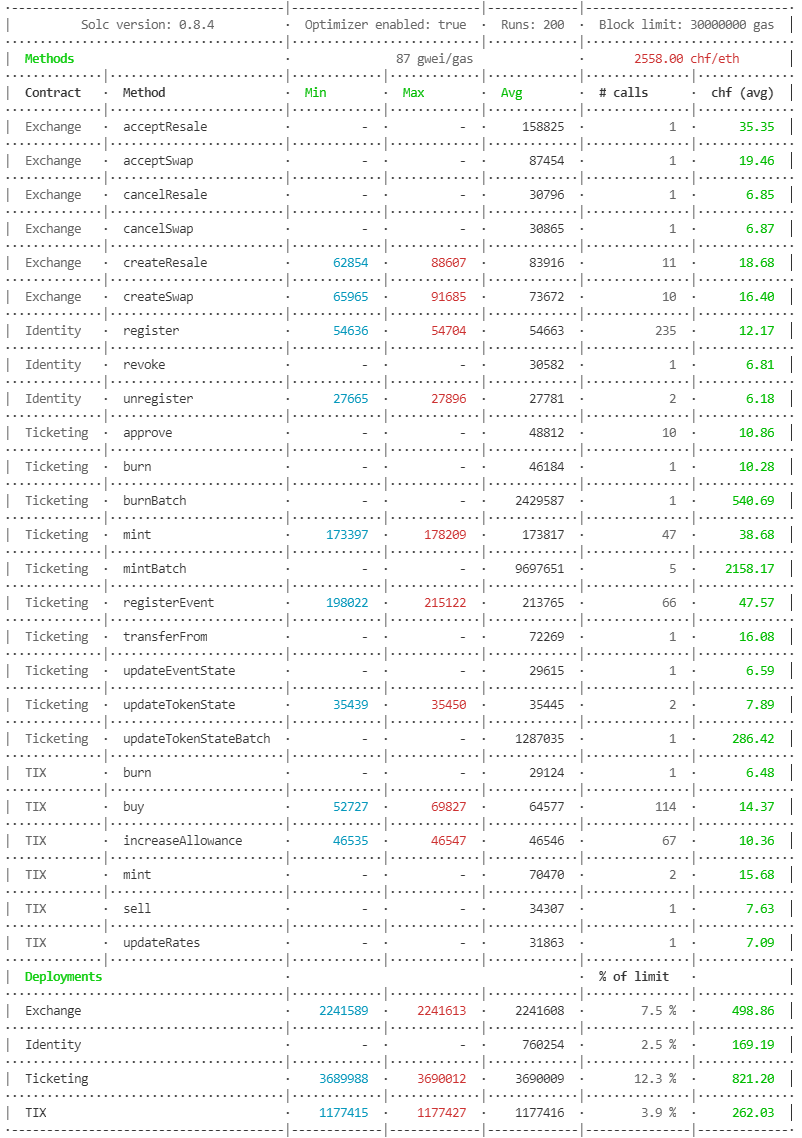
\includegraphics[width=\textwidth]{marketplace_price_ethereum_01_02_2022.PNG}

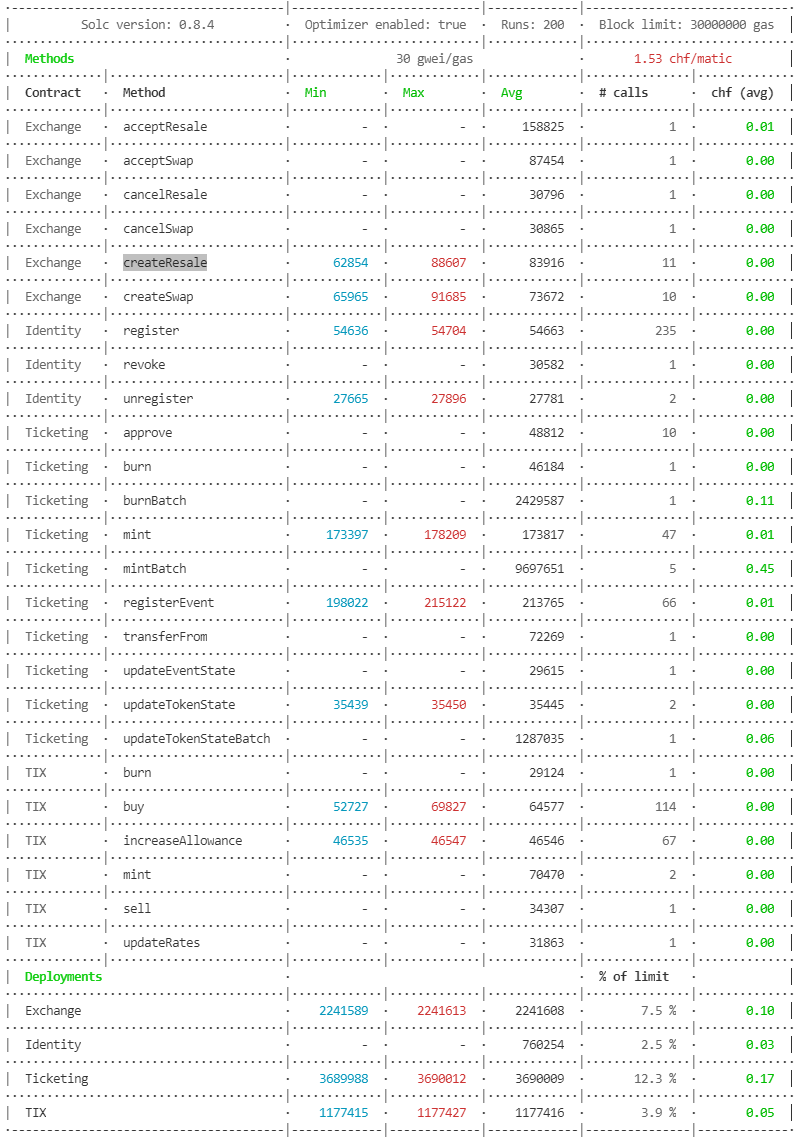
\includegraphics[width=\textwidth]{marketplace_price_polygon_01_02_2022.PNG}

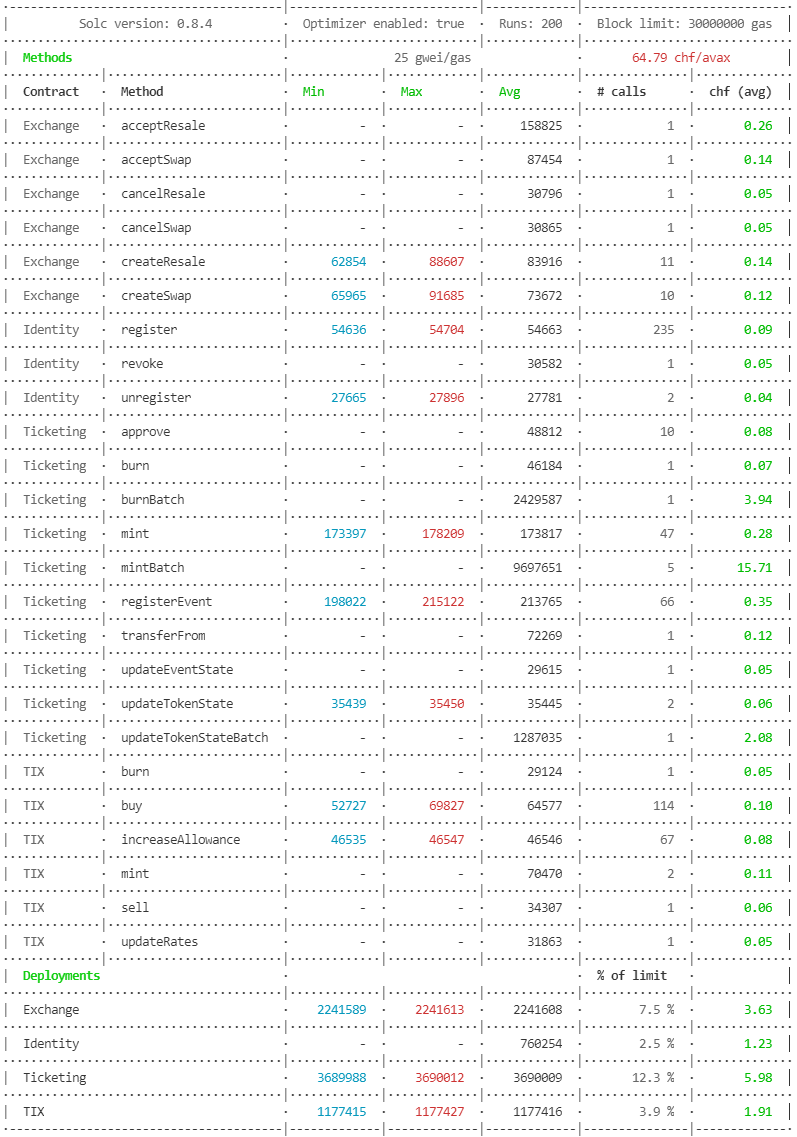
\includegraphics[width=\textwidth]{marketplace_price_avalanche_01_02_2022.PNG}

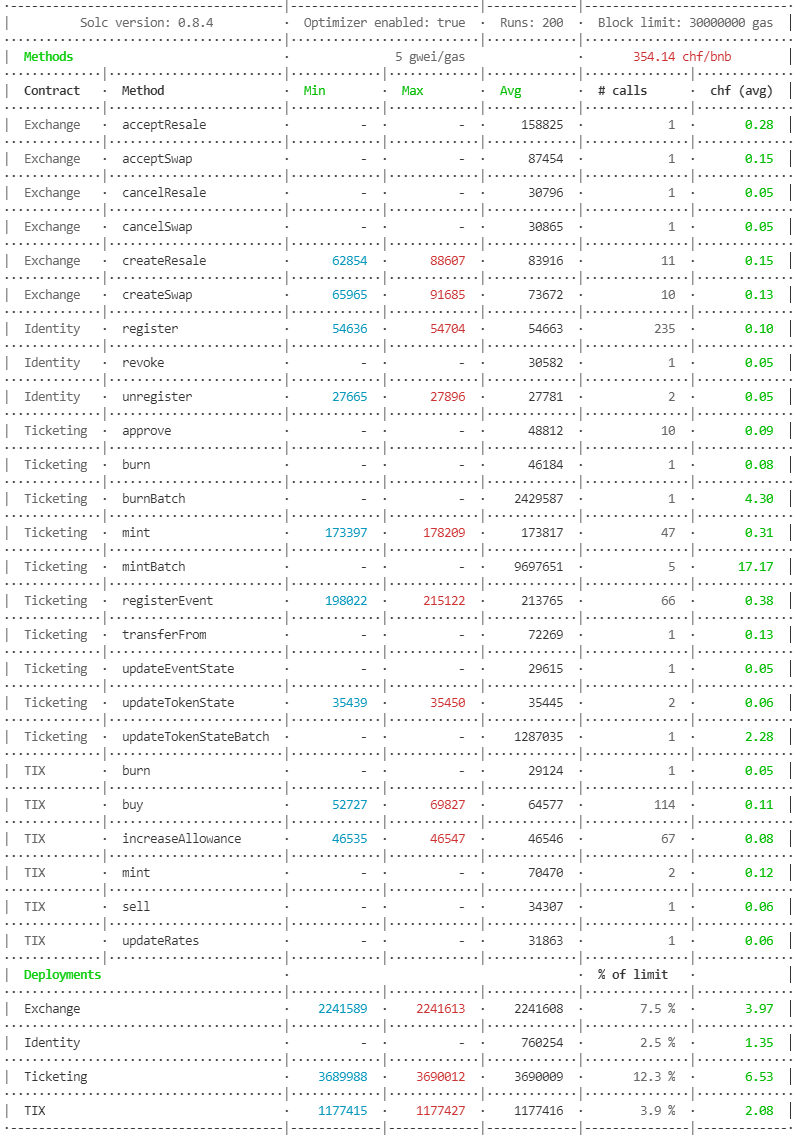
\includegraphics[width=\textwidth]{marketplace_price_binance_01_02_2022.PNG}

Additional costs induced by the signature (Measured done the 01.02.2022):

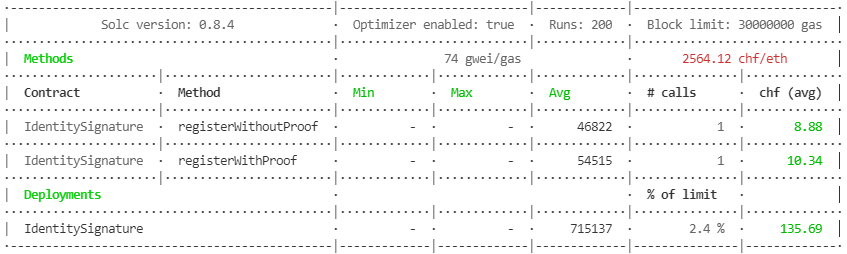
\includegraphics[width=\textwidth]{identity_sig_price_overhead_ethereum_01_02_2022.PNG}

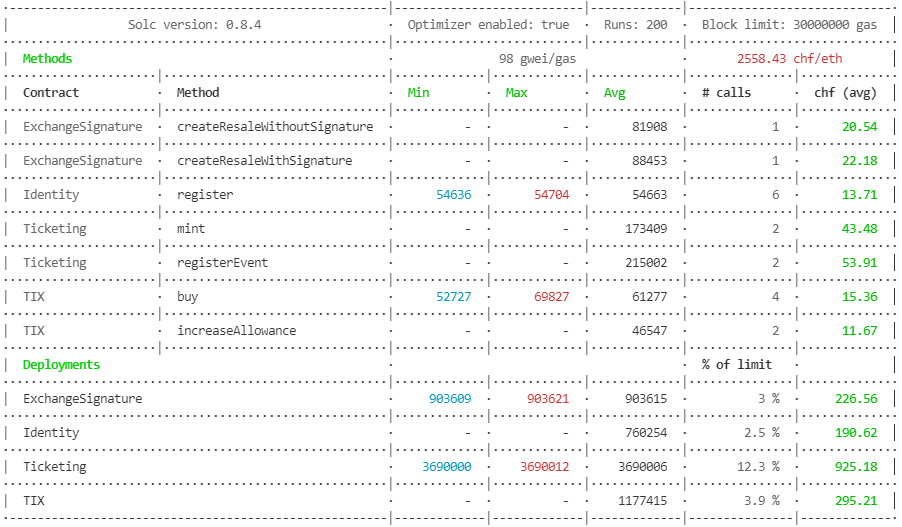
\includegraphics[width=\textwidth]{exchange_sig_price_overhead_ethereum_01_02_2022.PNG}

%%%%%%%%%%%%%%%%%%%%%%
\chapter{Limitation and future work}
%%%%%%%%%%%%%%%%%%%%%%

\section{Design optimization}
Although the implementation shows that the design works, there is one point that is not satisfactory. When a spectator creates a resale offer, he must make two transactions. The first transaction authorizes the exchange contract to transfer the spectator's ticket. The second transaction creates the resale offer. The spectator who buys the ticket in resale must also make two transactions. The first gives the authorization to the Exchange contract to transfer the TIX and the second transaction accepts the resale offer.

The reason why it is necessary to make two transactions is linked to the operation of the ERC721 and ERC20 standard. To transfer an asset, you must either be the owner or have received the approval of its owner. Once the transfer is complete, the approval is withdrawn.

One solution to this problem would be to have the TIX contract and the Ticketing contract white list the address of the Exchange smart contract so that it does not need to be given prior approval.
However, this approach is not a good idea because it blurs the line between the different smart contracts and their role. It opposes the blockchain philosophy which says that the end user must be the sole owner of these goods. Additionally, if the Exchange contract has a security hole, an attacker could potentially steal TIX. The principle of least privilege is not respected with this approach.

Here we propose an approach that might work. The idea is to use cryptography so that spectators can create off-chain evidence that authorizes the Exchange contract to transfer TIXs and tickets on their behalf. We also need to modify the ERC721 and ERC20 standards so that it accepts this new type of approval. Note that there is nothing new to build. We can construct proofs in the same way as those created by oracles. And the proof checking mechanism that is used to check proofs from oracles can be integrated into both standards to support this new type of approval. As with this approach it is no longer necessary to give the approval to transfer the TIX and the tickets, we halve the number of transactions to be made to carry out a resale.

We can go even further in the process by needing to make a single transaction to make a resale. With the current design, when a viewer resells a ticket, they first ask the oracle to create proof of resale approval. Once he has this proof, he lists his ticket on the Exchange smart contract by creating a resale offer. However, it is not necessary to list the offer directly on the smart contract. This can be done off-chain in order to save a transaction. To do this, the seller must create a proof of resale authorization in the same way as the Approver oracle. This proof can then be used by a buyer to redeem the tickets.

If we combine the two approaches, we offer the possibility of reselling a ticket by making a single transaction. Here is a high level description of the flow. The seller asks the oracle to create proof of resale approval. The seller creates two proofs. Proof of Resale Approval that authorizes a buyer to purchase their ticket and Proof of Transfer Approval that authorizes the Exchange Contract to transfer the ticket on their behalf. The buyer creates proof of transfer approval that authorizes the Exchange contract to transfer the TIX on their behalf. Finally, the seller creates a redemption transaction for the ticket that contains the four proofs and sends it to the blockchain. The smart contract checks that all authorizations are valid and executes the redemption operation.

To go even further in the process, we could also aggregate the proofs into one in order to reduce the complexity of the verification of the proofs on the smart contract and therefore the transaction execution costs. To do this, we need to construct proofs that have homomorphic properties.


TODO: COMPARAISON DES DEUX APPROCHES: la première (si on enleve l'oracle) permet de créer une place de marché non régulé mais entièrement decentralisé, la deuxième permet de créer une place de marché réguler et plus pratique mais pas totalement decentralisé (cela peut être le cas avec des oracles decentralisés)
La business logique on-chain est aussi beaucoup plus simple
Le swap est modifié car il ne faisait pas sens. Le swap doit être peer to peer uniquement.

TODO: clarify that the optional buyer is used for P2P resale and a resale with an empty optional buyer is meant to be listed on the marketplace

TODO: explain how to enable off-chain payment with strip and signature

TODO: explain it prevents someone to create a resale and then remove the approval on the token so that the transaction fails.

TODO: conclure en disant que l'approche V1 et l'approche V2 sont deux exemples et qu'il y a plein d'autre approche possible en terme de flow, custodialité et decentralisation. 

\section{Time-based proof expiration}
TODO

Check that a timestamp is below a threshold like time-based transfer rules

\section{payment splitter}
TODO

To better manage the splitting of money during the resale process and reduce the number of tix transfer proof

\section{Proof of ownership and scanner oracle}
An aspect that has not been addressed in this thesis is the management of the QR code that is scanned at the entrance of the event. TIXnGO uses encrypted QR codes which are revealed before the start of the event. The activation of the QR code can be done using bluetooth beacons. When the phone receives the signal from the beacon, it reveals the QR code. This can also be done with a time based activation. In this case, the QR code is activated a few hours before the start of the event.

The problem with this approach is that the QR code and the decryption key must be permanently stored on the user's phone because it is possible that the user is not able to access the internet once outside the entrance. Often, the quality of the mobile network is degraded because there are many people. Although it is possible to store the private key in the phone's secure enclave and extensively test the application code to ensure that it is very difficult to extract the QR code and use it at malicious purposes, this approach is not optimal.

Another approach is to generate a QR code that depends on the ticket owner, i.e. if two people had the same ticket, they would see a different QR code. With this approach, it is not necessary to encrypt the QR code. This approach is relatively easy to set up and has already been tested by AlphaWallet. The approach consists in generating a proof of ownership attesting that the person holds the ticket. To do this, the person proves that he is the owner of the address holding the ticket. The proof is then used to construct the QR code. You can find more info here\footnote{https://medium.com/opensea/cryptotickets-the-first-blockchain-based-tickets-are-live-on-opensea-5a29d0223c3d}.

\section{Decentralized oracles}
As we mentioned above, oracles are centralized. This is not a good thing because it creates a single point of failure, it opens the door to censorship and it goes against the philosophy of decentralization. To overcome these problems, we could use a decentralized oracle such as Chainlink.

\section{Performance test on zkSync or StarkNet}
The zk rollups, which in my opinion are the future of blockchain scalability, are becoming increasingly popular. It would be interesting to see how well the system would perform and what changes would need to be made to the system in order to make it work on these layer 2.

\section{TIX token features}
For the moment, the TIX token has very little use and it could perfectly be replaced by ETH. Here are some ideas that might make it more useful.

The TIX could be used as a governance token so that users can vote for new features in the application. For example, it would be possible to make a vote to determine if the spectators would like to have the possibility of claiming the souvenir ticket of an event in the form of NFT. The governance could also let the organizers vote for the next features they would like the development team to implement first.

It would also be possible to create a reward pool that can be shared regularly between the most acidus users of the application or to people who discover security flaws in the system. The pool could be filled by taking a small commission on each resale of tickets.

TODO: instead of a token we can also emit a tokenized security with the help of Taurus

TODO: exchange with liquidity to buy back tickets in exchange of TIX. This could be a good incentive to fight black market and side channel payment.

TODO: list potential on-chain rules: limit the number of ticket hold by single spectator by event, etc

%%%%%%%%%%%%%%%%%%%%
\chapter{Conclusion}
%%%%%%%%%%%%%%%%%%%%

\textit{In the conclusion you repeat the main result and finalize the discussion of
your project. Mention the core results and why as well as how your system
advances the status quo.} \\

\cleardoublepage
\phantomsection
\addcontentsline{toc}{chapter}{Bibliography}
\nocite{*}
\printbibliography

\appendix
%%%%%%%%%%%%%%%%%%%%%%%%%%%%%%%%%%%%%%
\chapter{List of events}
%%%%%%%%%%%%%%%%%%%%%%%%%%%%%%%%%%%%%%
\label{sec:appendix_a}

The structure of an event is the following: 
\begin{verbatim}
EventName(typeOfFirstElt nameOfFirstElt, typeOfSecondElt nameOfSecondElt, ...)
\end{verbatim}



\paragraph{Identity}
\begin{verbatim}
Registation(address user, bytes32 class, bytes32 hash, bytes signature);
Unregistration(address user);
Revocation(address user);
\end{verbatim}

\paragraph{TIX}
\begin{verbatim}
Purchase(address user, uint256 amount);
Sale(address user, uint256 amount);
Transfer(address from, address to, uint256 value);
Approval(address owner, address spender, uint256 value);
\end{verbatim}

\paragraph{Ticketing}
\begin{verbatim}
EventRegistration(uint256 eventId, address owner);
EventUpdate(uint256 eventId, bytes32 state);
Minting(uint256 tokenId, uint256 ticketId, address owner);
Burning(uint256 tokenId, uint256 ticketId);
TokenUpdate(uint256 tokenId, bytes32 state);
Transfer(address from, address to, uint256 tokenId);
Approval(address owner, address approved, uint256 tokenId);
\end{verbatim}

\paragraph{Exchange}
\begin{verbatim}
CreateResale(uint256 tokenId, uint256 price, address optionalBuyer);
CancelResale(uint256 tokenId);
AcceptResale(address seller, address buyer, uint256 tokenId, uint256 price);
CreateSwap(uint256 tokenId, uint256 eventIdOfWantedToken, address optionalParticipant);
CancelSwap(uint256 tokenId);
AcceptSwap(address creator, address acceptor, uint256 creatorTokenId, 
           uint256 acceptorTokenId);
\end{verbatim}

\end{document}